\chapter{Optical Character Recognition}
\label{ch:OCR}

Optical character recognition (OCR) is a branch of digital image processing. Its aim is to detect and convert a text on an image into a machine-readable text. This discipline can be divided into three similar, yet different tasks: reading text on scanned printed documents, reading of handwritten texts and scene text recognition (also called text in the wild). The first task is very well developed, first successful results date back to the second half twentieth and were used in commercial sector \cite{ocrhist}. If we assume the handwritten text is on scanned single colored paper or created using a digital pen and that it was written legibly and without omitting letters in words due to fast writing, then recognition is similar to printed documents. The last task -- scene text recognition (STR) is the most challenging one. 
The main factors that make STR a more difficult task are listed below.\cite{chen2021text, raisi2020text}

\begin{itemize}
    \item Complex background: in scanned documents background is white and without  a distinctive pattern (omitting lines is an easy preprocessing task), while in scene images there are objects that can be mistaken for letters.
    \item Text diversity: text can appear in various colors, fonts, sizes or orientations.
    \item Distortions: photographs often suffer from noise due to bad illumination, also from motion or out-of-focus blurring, perspective distortion due to the capturing angle. Other problems come from the insufficient resolution that might be set on the camera.
\end{itemize}

Apart from these main categories of image text data there exist born-digital images (e. g. web advertisements or any cases where text was digitally added on images or videos) and poster/newspaper images. These share with scene images the diversity of text but are free from visual distortions caused by cameras. Examples of different image data are in sections \ref*{sec:datasets} and \ref*{sec:expDatasets}. 

Digital reading of a text on an image consists of two main tasks -- text detection and text recognition. Both processes are described in the next sections.

\section{Text Detection}

The first phase of digital text processing is to detect the text regions on the image. The goal is to determine a bounding box surrounding a group of letters -- usually one word, but it can be also a text line consisting of few words. This box may be a bounding rectangle or a polygon which is more accurate for curved or skewed text. It is ideal when the bounding box contains the letters with as little background as possible. The methods store this information as a set of coordinates which unambiguously define the box, some methods produce cropped images based on the coordinates or a binary image with highlighted detected area.% When text candidates are found they have to be verified.
Methods used for text detection can be categorizes into formerly used classical machine learning methods and deep learning methods. 

\subsection*{Classical Methods}

Classical methods include connected component methods and sliding window methods. In the latter method an image is scanned with a moving window of certain size. In each position of the window features are computed, for example, standard deviation or histogram of oriented gradients and are compared with values known from training images with text.    This approach does not have a good response for scene images, because many objects can be misunderstood as letters and vice versa. Connected component based methods extract from the image features like color, texture, edges or corners. Then they are classified either as text or non-text by a traditional classifier such as support vector machines, nearest neighbor or random forest. Detected letters are then combine into words or text lines if desired \cite{raisi2020text}. Classical methods are generally not very successful with scene images where most of the observed values are negatively influenced by distorting factors listed above. In recent years the development of neural networks enabled a new, efficient way of detecting text in images.

\subsection*{Deep Learning Methods}

Deep learning methods are faster, more precise than the classical methods. They are automated and need less of human assistance therefore they can process bigger amounts of data. Another advantage is that algorithms can be generalized and used for other image detection tasks. Most of the state-of-the-art methods utilize convolutional neural network (CNN). Deep learning methods can be split into bounding-box regression based, segmentation based and hybrid methods according to the survey of Raisi et al.\cite{raisi2020text}.

Bounding-box regression based methods treat text as an object and predict directly the bounding box around text. However, the bounding boxes have different aspect ratio than typical objects, because text is usually long and thin. Some methods decompose the text on smaller units and concentrate on distances between the units. These methods are hard to tune during training an usually fail on distinctly curved text. Examples of bounding-box methods are TextBoxes \cite{liao2017textboxes}, TextBoxes++ \cite{liao2018textboxes++} or EAST \cite{zhou2017east}. Segmentation based methods investigate the image at pixel level. The image data are processed by a CNN which produces a segmentation map from which a bounding box is generated. An example of this method is PSENet \cite{wang2019shape}. Hybrid methods combine the features obtained by regression and the segmentation map from CNN. The segmentation methods tend to return false positive detection. They select pixels that are not text at the borders of letters or when there is a complicated background. Hybrid methods further process the results from segmentation and precisely detect text. Example methods are PMTD \cite{liu2019pyramid}.

A popular method in recent years is Character Region Awareness for Text Detection -- CRAFT. This method in contrast to the previously mentioned methods detects text based on character level rather than word (group of characters) level. CRAFT trains a CNN which produces two results for a character -- a region score and an affinity score. Because this method goes over individual characters it performs very well on curved and deformed text and outperforms 15 popular detection methods according to the authors of CRAFT in their paper \cite{craft2}.


\section{Text Recognition}

Text recognition converts a detected text on an image to a string. Analogous to detection methods again recognition methods can be divided to classical methods and deep learning methods. Traditional methods work with image features such as histogram of gradients, features from SIFT\footnote{Scale-Invariant Feature Transform}, which are then classified by SVM or nearest neighbor algorithms. Moreover methods can be divided on segmentation-based and segmentation free methods. The former classify single characters gradually and then connect them into a word. The latter examine the text line as a whole, so it can use word neighborhood for contextual information. In the following subsection four stages of segmentation free methods are described.\cite{chen2021text,raisi2020text}

\subsection*{Segmentation Free Methods}

Segmentation free methods follow a pipeline with four stages: image preprocessing, feature representation, sequence modeling and prediction.

\begin{enumerate}
    \item \textbf{Image Preprocessing Stage}: during this phase visual quality of the image is improved as much as possible. Because in scene images background is usually not a plain color, but a complex mixture of colors in various shape, the effort is to replace it and create optimally a binary image with one color for the foreground text and another for the background. It can be achieved by using neural networks. If complete background removal is not easily achievable, basic image preprocessing such as noise removal are performed at least. Optional enhancement for scene images is to increase readability via superresolution, this removes noise caused by low resolution of the original image. If the text is perspectively distorted or curved there is an effort to straighten the text, this process is called rectification. It is a computationally expensive process, therefore it is not used very often.\cite{chen2021text}
    \item \textbf{Feature Representation Stage}: now it is necessary to extract features from the image data that are used as a representation of objects (text) in the images. For this purpose CNNs are widely used. For example namely these types VGGNet, ResNet, DenseNet, recurrent CNN (RCNN).
    \item \textbf{Sequence Modeling Stage}: An optional step between final prediction and features. A contextual information is obtained via a recurrent neural network. Mostly one of two types called long short-term memory (LSTM) and bidirectional long short-term memory (BLSTM) is applied. The information is utilized  during the last stage for predicting subsequent characters rather then predicting each character individually. 
    \item \textbf{Prediction}: in this last stage the model returns a target word or text line that was recognized. Two major technologies are connectionist temporal classification (CTC) and the attention mechanism. 
    Because some letters span more than others it may happen that the letter is classified multiple times, to avoid this CTC introduces a blank symbol and inserts it among characters in various locations and creates character sequences. CTC then trains the network to maximize the probability distribution over all possible sequences. This approach is to a great extent dependent on a lexicon or language information about word formation. Attention-based methods utilizes RNNs \cite{ctc}. "The attention mechanism learns the alignment between the input instance image
    and the output text sequences by referring to the history of the target characters and the encoded
    feature vectors" \cite[page 12]{chen2021text}.
\end{enumerate}



% \subsection*{Classical Methods}
% Traditional methods work with image features such as histogram of gradients, features from SIFT\footnote{Scale-Invariant Feature Transform}, which are then classified by SVM or nearest neighbor algorithms. These methods 
% \subsection*{Deep Learning Methods}


% various scripts... popsat nekde...!!!

\section{Datasets}
\label{sec:datasets}

Optical Character Recognition requires data as any other machine learning task. Data are usually divided in two main types - scene and synthetic. Scene datasets contains photographs of real world objects and sceneries where some text occurs, for example shop signs, road signs or car plates. Synthetic dataset are automatically generated images where words are chosen from a extensive dictionary, a font is picked for each word and some sort of deformation is applied. It can be a text distortion to make the text curved or projectively altered, as well as blurring or lighting changes that make the text less obvious for the detector.

Synthetic datasets are usually used for training the models, because it is easier to generate millions of synthetic images rather than to take even one hundredth of a such number of photographs. Needless to say that when generating an image, the ground truth is known and can be saved during the generation process while photographs have to be manually labeled which takes time and might be inaccurate or automatically labeled which also often leads to many mistakes. Scene datasets are then used for testing purposes or for fine tuning a pretrained model.

In this paragraph sample datasets are introduced. To begin with synthetic dataset MJSynth is a very important dataset because it consists of almost 9 million images covering 90,000 English words. It includes data only for recognition which means that one image has only one word and border of the image  represents the word bounding rectangle.\cite{mjsynth}. Another synthetic dataset is called SynthText and contains 800 thousand images with approximately 8 million word instances written on the images \cite{synthtext}. Three scene text datasets were created for International Conference on Document Analysis and Recognition (ICDAR) competition. Sets ICDAR03, ICDAR13 and ICDAR15 were used in competitions in years 2003, 2013 and 2015, respectively. First two ICDAR datasets include only horizontal text, text of various orientation appears  in set from 2015 \cite{raisi2020text}. Another widely used dataset is The Street View Text (SVT) which contains images with text harvested from Google Street View \cite{svt}. SVT and most other scene text datasets offers mainly frontal text with minimal perspective distortion. However, perspective text is frequent in real life applications of OCR for example previously mentioned street photographs, where it is impossible to capture every visible text from frontal view. Thus Phan et. al \cite{svtp} created a new StreetViewText-Perspective derived from SVT, it shows the same places as SVT but from different perspective. Another dataset CUT80 focuses on curved text as well as CTW1500 dataset. For text recognition there exist for example IIIT5k dataset containing 5000 cropped images harvested from Google image search. It combines both scene text images and born-digital images \cite{IIIT}. One of the most widely used dataset is COCO-Text which includes over 60,000 images with almost 250,000 word instances \cite{coco}.

Datasets that were used for comparison of detection and recognition methods, namely, SCUT-CTW1500 dataset, Kaist Scene Text Database, Born-Digital Images, are described in more detail in Chapter \ref{ch:testing}. 

\section{Evaluation}
\label{sec:eval}

\subsection*{Text Detection}
A detection model tries to detect a text regions as precise as possible. It predicts a bounding box around the text and return its coordinates. As said earlier it can be an irregular polygon or a rectangle.
% In experiments performed in this thesis I used results only in the rectangular shape, therefore I will concern in this section only this case.

For measuring the performance of a detection model in general object detection a intersection over union (IOU) is used and it can be evenly applied on text detection. The principle is to compute the intersection of a ground truth bounding box and predicted bounding box and divide it by union of those two areas.\cite{pyimage_iou}

\begin{figure}[hbtp]
    \centering
    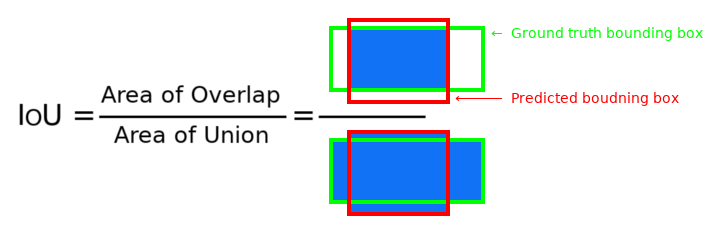
\includegraphics[scale=0.4]{obrazky/iou_equation.png}
    \caption{Iou formula with a bounding box visual interpretation.}
    \label{Im:iou}
\end{figure}

\subsection*{Text Recognition}
To test how much is the recognition model successful various evaluation metrics were created. The simplest that comes to a mind is compare the word in the image with the predicted one. We can either compare words strictly and as correct classify only when all characters match and even a small mistake makes the prediction false, or we can use  the metric called word error rate (WER). Before we define how it is computed, we must introduce three types of error that are taken into account:
\begin{itemize}
    \item \textbf{substitutions}: words with one or more misspelled characters,
    \item \textbf{insertions}: words that were added (do not appear in original text),
    \item \textbf{deletions}: missing words.
\end{itemize}

WER is then defined as follows.
\begin{equation}
    WER = \frac{(i_w + s_w + d_w)}{n_w},
\end{equation}
where $i_w$ is the number of inserted words, $s_w$ is the number of altered words, $d_w$ is the number of lost words and $n_w$ is the number of all words in a ground truth text. The chosen value of WER is the one where the sum in numerator is minimal.\cite{cersite}

This approach is straightforward and it is a useful for long text, for example scanned books or documents. However, used on scene text or generally images with sparse text that does  not contain sentences, it has some drawbacks. Scene text images do not have a long contextual information, there are words that belong together (such as names of countries) but mostly there are street signs, telephone numbers, names of people or companies that do not occur in lexicon. In these cases it is often that the recognizer makes mistake in just one character, that can be barely legible due to an extravagant font or lighting conditions or other distortions. Therefore, it is better to focus on characters and validate each letter in a word separately. For this purpose is used, similar to word error rate, a character error rate (CER). There are again three possible error types -- substitution, insertion and deletion of a character in a word.

The formula for CER computations is also analogous
\begin{equation}
    CER = \frac{(i + s + d)}{n},
\end{equation}

where $i$ is the number of inserted characters, $s$ is the number of substituted characters, $d$ is the number of deleted characters and $n$ is the number of all characters in a ground truth word.\cite{cersite}

The sum of the three error operations is called a Levenshtein distance. Let $s$ be the ground truth (source) string and $t$ the predicted (target) string. The steps of the  algorithm are \cite{cerpaper}:
\begin{enumerate}
    \item Let $n$ be the length of $\bm{s}$ and $m$ the length of $\bm{t}$. Construct an empty matrix $\bm{d}$ with $0,\dots, n$ columns and $0,\dots, m$ rows.
    \item Initialize the first row to $0,\dots, n$ and first column to $0,\dots, m$.
    \item Go through $\bm{s}$ ($i=1,\dots,n$) and $\bm{t}$($j=1,\dots, m$).
    \begin{itemize}
        \item Compare $\bm{s}[i]$ and $\bm{t}[j]$: 
        \subitem if it equals, set $cost = 0$,
        \subitem if it does not, set $cost = 1$.
        \item Set $\bm{d}[i,j]$ equal to the minimum value of:
        \subitem $\bm{d}[i-1,j]+1$ (deletion),
        \subitem $\bm{d}[i,j-1]+1$ (insertion),
        \subitem $\bm{d}[i-1,j-1]+cost$ (substitution).
    \end{itemize} 
    \item Repeat step 3 until $\bm{d}[m,n]$ value is computed. That is the Levenshtein distance.
\end{enumerate}

It is clear that the number of mistakes can exceed the length of the source word, which leads to error rate larger than one hundred percent. For this purpose sometimes normalized CER is used. To obtain it the sum of errors is divided not by the number of characters in the source word but by the sum $(i+s+d+c)$, where $i,s,d$ are the error operations and $c$ is the number of correct characters the predicted word and can be computed as $c = n - d - s$. This way the denominator is always larger than the numerator (or equal). After modifications we get the following formula:
\begin{equation}
    CER = \frac{i+s+d}{n+i}=\frac{Levenshtein\ distance}{n+i}.
\end{equation}
